\subsection{Mission}

Au cours de mon stage, j'ai entrepris diverses missions au sein de l'association dans le but de mener à bien le projet qui m'a été confié.

Initialement, je vais détailler en profondeur le projet qui m'a été attribué, puis je vais fournir des explications approfondies sur les différentes tâches entreprises pour la réalisation réussie de ce projet.

\subsubsection{Le projet}

Le projet consiste en la création d'une application interne à l'école CY~Tech, visant à améliorer la communication des associations étudiantes concernant les événements qu'elles organisent. Cette application offre aux étudiants la possibilité de s'inscrire aisément aux événements et de rester informés plus facilement de ce qui se passe autour d'eux.

Le projet est subdivisé en deux sous-projets : le développement d'une application web et la création d'une API.

L'application web fait office d'interface graphique entre l'utilisateur et l'API, assurant la liaison entre la base de données et l'interface utilisateur. Nous avons fait le choix de diviser le projet en deux parties distinctes pour garantir une maintenance optimale des applications et permettre à plusieurs applications web de bénéficier de ce service.

Plusieurs fonctionnalités essentielles sont prévues pour les applications :
\begin{itemize}
	\item Création et gestion de comptes utilisateurs ;
	\item Abonnement aux associations ;
	\item Participation aux événements ;
	\item Création d'événements ponctuels ou récurrents.
\end{itemize}

Il est impératif que les applications soient hautement sécurisées, tout en garantissant une maintenance aisée et une extensibilité optimale.

% TODO : améliorer cette section pour y ajouter toutes les contraintes liés aux applications
Pour cela, de nouvelles contraintes liés aux développement des applications apparaissent.
Pour l'application web, celle-ci devra être basé sur le concept de Single Web Page. 
Pour l'API, celle-ci devra être réactive.

\subsubsection{Détails}

\paragraph{Les comptes utilisateurs}

Posséder un compte utilisateur est un élément clé lors de l'utilisation d'une application. Cela nous permet d'enregistrer nos préférences et stocker des informations par rapport au contenu proposer par l'application. Cependant, il faut faire attention de sécuriser correctement l'authentification pour éviter que quelqu'un d'autre utilise un compte qui n'est pas à lui.

Dans le but de renforcer la sécurité de notre système d'authentification, nous avons pris la décision d'adopter Keycloak, une plateforme spécialisée dédiée à cet effet. En effet, ce serveur exploite le protocole OpenID Connect (OIDC), lequel garantit un processus d'authentification sécurisé et robuste.

OpenID Connect (OIDC) constitue un protocole d'authentification construit sur la base d'OAuth 2.0, spécialement conçu pour sécuriser les échanges entre applications et services en ligne. Ce protocole permet à un utilisateur de s'authentifier au sein d'une application en utilisant son identité provenant d'un fournisseur d'identité tiers, tel que Keycloak. L'usage de tokens d'authentification renforce la couche de sécurité, améliorant ainsi la fiabilité et la performance du processus.

La gestion des tokens d'authentification au sein de Keycloak se déroule de la manière suivante. Keycloak commence par généré un token d'authentification lorsque qu'un utilisateur se connecte. Une fois que le token est généré et récupérer par l'utilisateur, celui-ci est renvoyé à chaque fois lors d'une requête vers l'application API. Avant que la requête ne soit éxécuté, Keycloak vérifie si l'utilisateur est bien authentifié et s'il a les droits pour faire la requête, et si c'est le cas la requête est éxécutée. Un autre avantage des tokens générés par  Keycloak est l'expiration des tokens, qui peret de ne pas avoir un token stocké trop longtemps sur son ordinateur sans que celui-ci ne soit utilisé. Enfin, Keycloak utilise le concept de Single Sign-On, ce qui signifie qu'une fois qu'un utilisateur s'est authentifié auprès d'une application, aucune nouvelle connexion ne sera requise lorsqu'il accède à d'autres applications sécurisées par Keycloak au sein de la même session.

En synthèse, Keycloak exploite le protocole OIDC pour gérer les tokens d'authentification, renforçant ainsi la sécurité et la convivialité de l'authentification pour les applications et les utilisateurs. Cette approche permet d'établir un environnement d'authentification centralisé et sécurisé, couvrant l'ensemble des applications développés à la Corpauration.

\begin{figure}
	\centering
	\begin{subfigure}{.45\textwidth}
		\centering
		
\includegraphics[width=0.40\textwidth]{assets/keycloak.png}
		\subcaption{Keycloak}
		\label{fig:keycloak}
	\end{subfigure}
	\begin{subfigure}{.45\textwidth}
		\centering
		\includegraphics[width=0.40\textwidth]{assets/openid.png}
		\subcaption{OpenID}
		\label{fig:openid}
	\end{subfigure}
	\caption{Technologies utilisées pour l'authentification}
\end{figure}

\paragraph{Abonnements aux associations}

Comme chaque association est différentes, nous nous sommes dit que chaque étudiants auront des préférences pour certaines associations ou d'autres. Un système d'abonnement sera alors créé, ce qui permettra aux étudiants d'avoir une meilleure expérience utilisateur et avoir plus facilement accès aux événements qui pourraient les intéréssé.

\paragraph{Participation aux événements}

Le fait de pouvoir participer à des événements à partir de l'application à deux intérêts : un pour les étudiants et un pour les associations.

Nous avons remarquer que lorsqu'il faut cliquer sur un lien pour remplir un formulaire d'inscription sur Google Form par exemple, les étudiants ne le remplisse pas toujours et moins d'étudiants viennent à nos événements. Pour contrer ce problème, simplifier l'inscription en centralisant tout sur une application et pouvoir remplir un formulaire d'inscription avec les informations qui est déjà dans la base de données sera plus simple. Les associations auront donc plus d'étudiants inscrits et un onglet pour voir tout les inscrits, et pour les étudiants ils pourront avoir accès directement aux événements auxquels ils se sont inscrit et définir un rappel pour ne pas l'oublier.

\paragraph{Création d'événements}

Créer des événements est la fonctionalité majeure de l'application. Le but est de pouvoir créer des événements le plus personalisable possible, tel que la possibilité de renseigner certains champs ou non, la possibilité de créer des événements périodiques et de tout pouvoir modifier comme on le souhaite.

\paragraph{L'application web}

Pour réaliser tout ces fonctionalités, il est plus simple d'utiliser une interface graphique. Nous avons donc décider de créer une application web afin de pouvoir bénéficier de toutes les fonctionalités le plus facilement possible.

Nous avons donc décider d'utiliser le célèbre framework Javascript Vue et la librairie de composants open-source Vuetify.

Vue est un framework JavaScript progressif et performant destiné à la création d'interfaces utilisateur interactives et dynamiques. Il facilite le développement en fournissant une structure organisée pour construire des applications web à travers la composition de composants réutilisables. Vue met l'accent sur la réactivité des données, ce qui signifie que les changements dans l'état de l'application sont automatiquement reflétés dans l'interface utilisateur sans nécessiter de manipulation directe du DOM.

Vuetify, quant à lui, est une bibliothèque de composants visuels pour Vue.js, conçue pour simplifier la création d'interfaces utilisateur esthétiques et réactives. Vuetify fournit un ensemble complet de composants pré-conçus, tels que des boutons, des barres de navigation, des cartes, et bien plus encore. Ces composants peuvent être facilement intégrés dans des projets Vue pour accélérer le processus de développement et garantir une cohérence visuelle dans toute l'application. En utilisant Vuetify, nous pouvons rapidement créer des interfaces modernes et attractives sans avoir à concevoir chaque élément visuel à partir de zéro.

L'application web ne va pas dialoguer directement avec la base de données, mais plutôt avec une API qui contiendra tout le dialogue avec la base de données.

\begin{figure}
	\centering
	\begin{subfigure}{.45\textwidth}
		\centering
		
\includegraphics[width=0.40\textwidth]{assets/vue.png}
		\subcaption{Vue}
		\label{fig:vue}
	\end{subfigure}
	\begin{subfigure}{.45\textwidth}
		\centering
		
\includegraphics[width=0.40\textwidth]{assets/vuetify.png}
		\subcaption{Vuetify}
		\label{fig:vuetify}
	\end{subfigure}
	\caption{Technologies utilisées pour l'application web}
\end{figure}

\paragraph{L'API}

\begin{figure}
	\centering
	\begin{subfigure}{.45\textwidth}
		\centering
		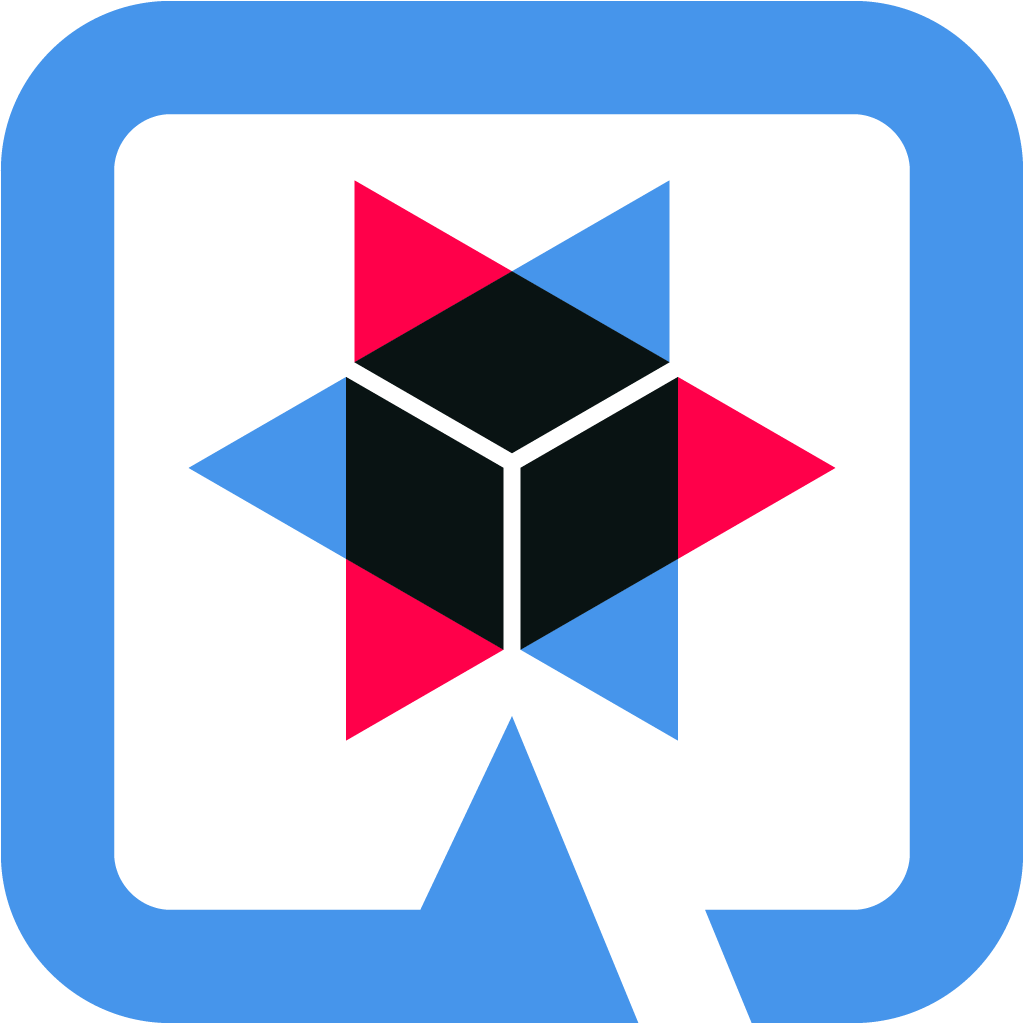
\includegraphics[width=0.40\textwidth]{assets/quarkus.png}
		\subcaption{Quarkus}
		\label{fig:quarkus}
	\end{subfigure}
	\begin{subfigure}{.45\textwidth}
		\centering
		
\includegraphics[width=0.40\textwidth]{assets/hibernate.png}
		\subcaption{Hibernate}
		\label{fig:openid}
	\end{subfigure}
	\caption{Technologies utilisées pour l'API}
\end{figure}

